\section{On-demand Provisioning for Simulation Workflows}
\label{previous:ondemand}

\citeauthor*{provisioning:ondemand} identify requirements that need to be addressed to make the current approach for scientific workflows used by the SimTech SWfMS more suitable for scientific simulation work~\autocite{provisioning:ondemand}.
These requirements are: Dynamic allocation as well as release of computing resources, on-demand provisioning and deprovisioning of workflow middleware and infrastructure, and dynamic deployment and undeployment of simulation services and their software stacks.
To fulfill these requirements, they propose a new service binding strategy that supports dynamic service deployment, an approach for dynamic provisioning and deprovisioning of workflow middleware, an architecture that is capable of these dynamic deployment and provisioning operations, and, as part of this architecture, the bootware - the subject of this diploma thesis - that kicks of these dynamic processes~\autocite{provisioning:ondemand}.

\begin{figure}[!htbp]
	\centering
	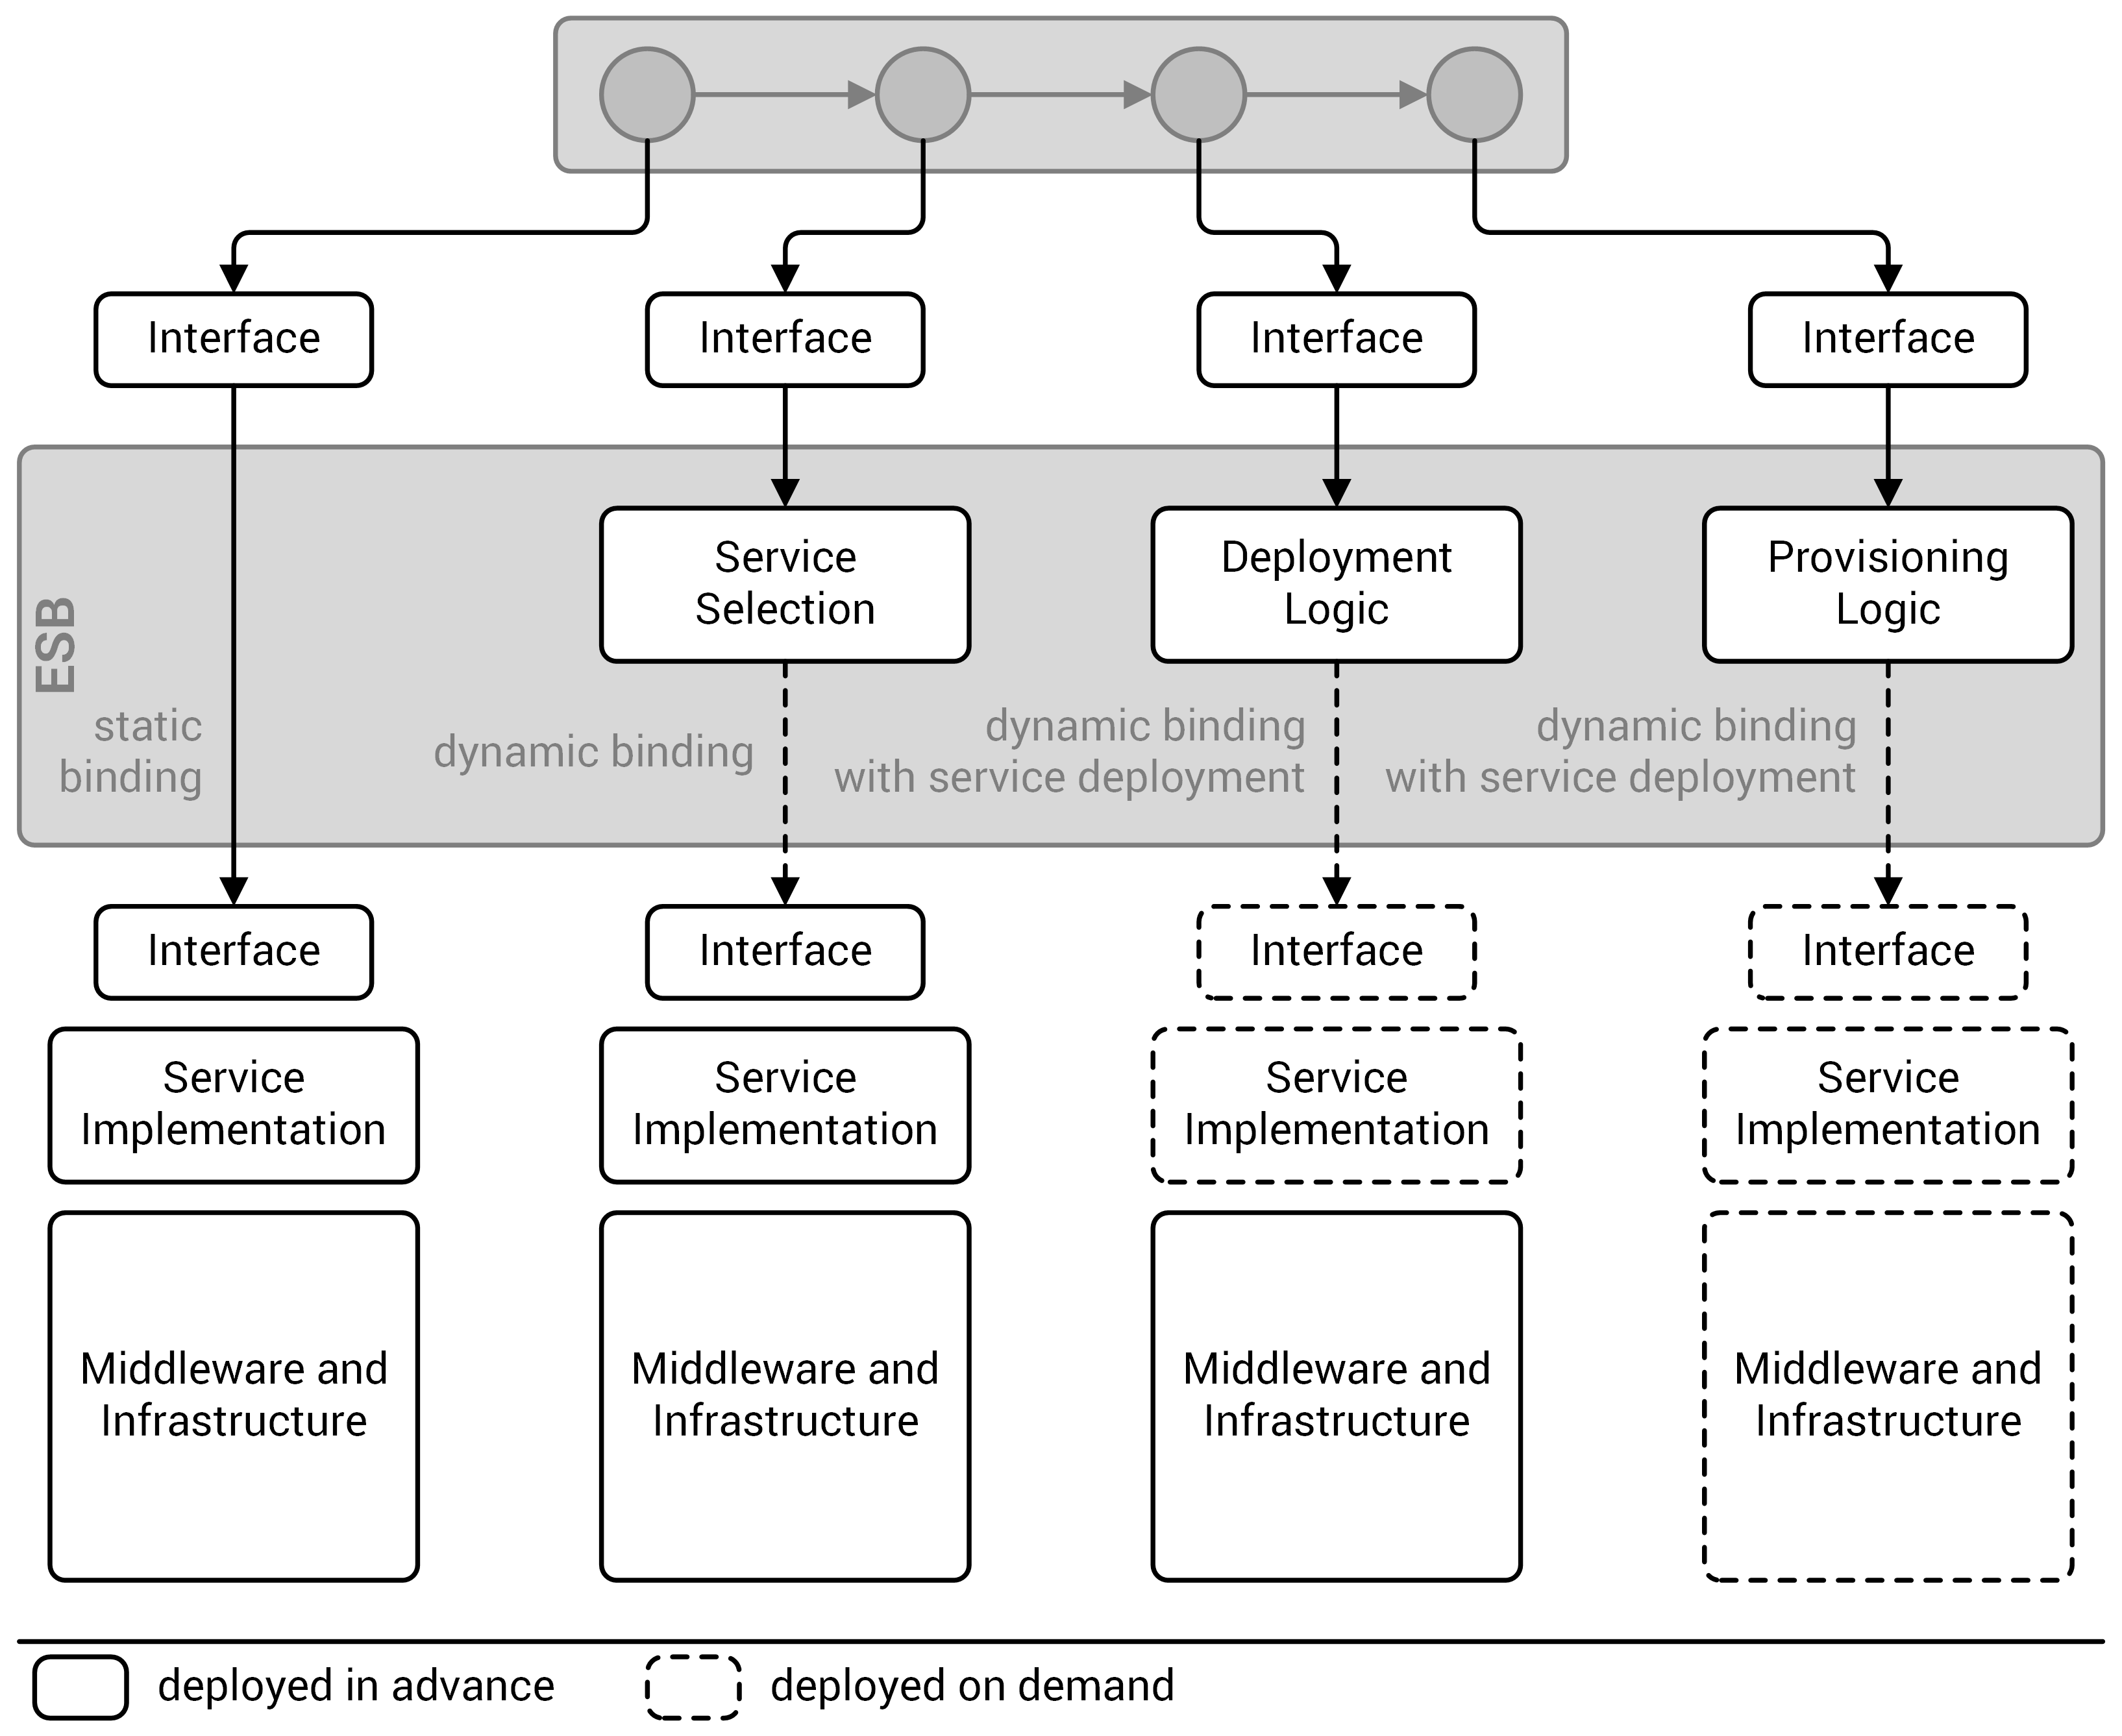
\includegraphics[resolution=600]{previous/assets/service_binding_strategies}
	\caption{Simplified overview of service binding strategies~\autocite[based on][]{provisioning:ondemand}.}
	\label{image:service_binding_strategies}
\end{figure}

The new service binding strategy is necessary, because existing static and dynamic binding strategies, as shown on the left and in the center of \autoref{image:service_binding_strategies}, rely on services that are always running, or, as in the case of dynamic binding with service deployment, only dynamically deploy the service, but not its middleware and infrastructure.
The new service binding strategy, shown on the right of \autoref{image:service_binding_strategies}, called \textit{dynamic binding with software stack provisioning}, is similar to the already existing dynamic binding with service deployment strategy, but adds the dynamic provisioning of the middleware and infrastructure required by the service~\autocite{provisioning:ondemand}.

Their approach for dynamic provisioning and deprovisioning of workflow middleware an simulation services is separated into six steps.
The first step is to model and start the execution of a simulation workflow.
For this, the Modeler component shown on the left of \autoref{image:original_architecture} is used.
In the second step, the middleware for executing the worklfow, e.g. the SWfMS, and its underlying infrastructure are provisioned.
This is shown in \autoref{image:original_architecture} as deployment step one and two.
In deployment step one, the bootware deploys a provisioning engine into a cloud environment.
In deployment step two, this provisioning engine is used to deploy the actual middleware.
Now, the workflow can be deployed on this middleware, which is step three.
In step four, an instance of this workflow is executed.
During this execution, some external service might be required that are not yet available.
The ESB determines this by checking the service registry.
If the requested service isn't available, the ESB tells the provisioning engine to provision this service.
The on-demand provisioning of services is step five, which corresponds to deployment step three in \autoref{image:original_architecture}.
The service is also deprovisioned if it is no longer needed.
The final step is to deprovision the workflow model and the workflow execution middleware after the execution of the workflow instance is finished~\autocite{provisioning:ondemand}.

\begin{figure}[!htbp]
	\centering
	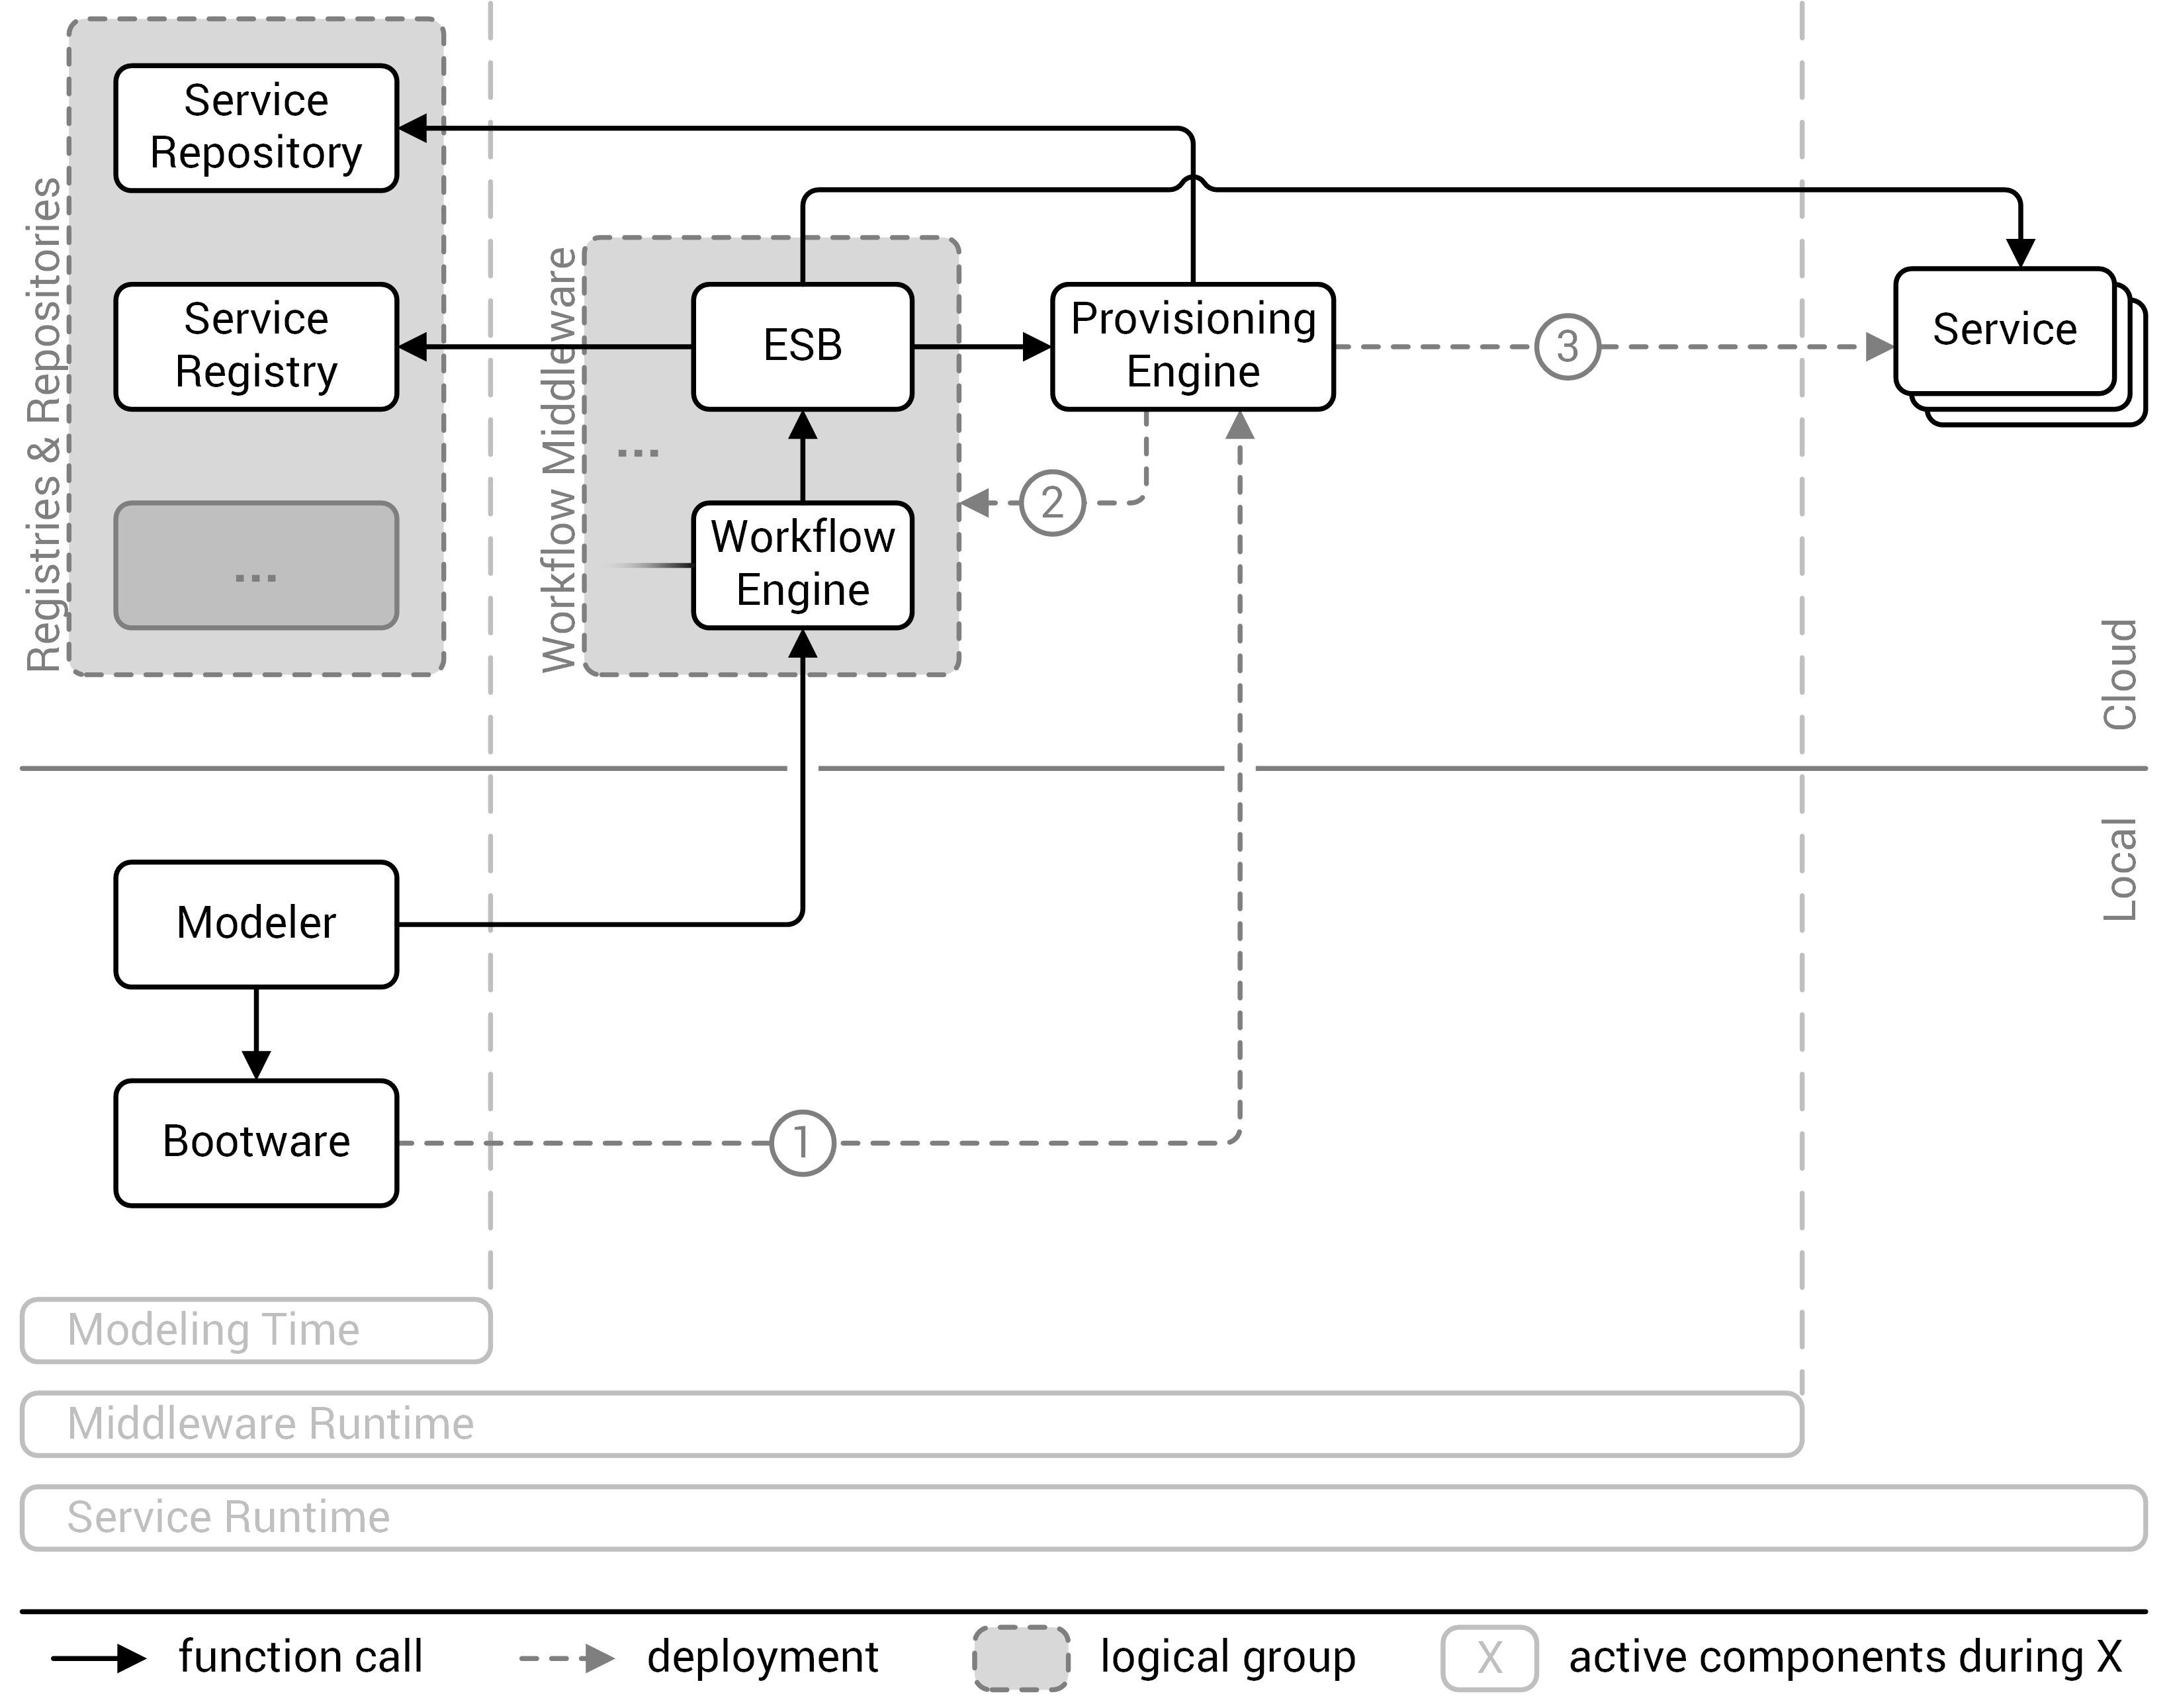
\includegraphics[resolution=600]{previous/assets/original_architecture}
	\caption{Proposed architecture~\autocite[based on][]{provisioning:ondemand}.}
	\label{image:original_architecture}
\end{figure}

The architecture they present can be separated into a local part and a cloud part, as well as different phases.
\autoref{image:original_architecture} shows that the only local components are the modeler and the bootware, while all other components are hosted in the cloud.
In the modeling phase, a scientist uses local modeling and monitoring tools in combination with cloud hosted repositories and registries to create a workflow.
These components are always running.
When he starts the execution of the the workflow, the local bootware component kicks of the on demand provisioning process and therefore the second phase, called middlware runtime phase.
In this phase, the bootloader deploys a provisioning engine in the cloud, which in turn deploys the workflow middleware.
Once the middleware is up and running, the workflow can be executed. During the execution, the ESB receives service calls from the workflow engine.
Services that are not running at this time can then be provisioned by the provisioning engine.
This takes place in the third phase, the service runtime phase.
The bars at the bottom of \autoref{image:original_architecture} show, which components are active during which phase~\autocite{provisioning:ondemand}.
